\documentclass[../ala_hataile.tex]{subfiles}
\begin{document}
\clearpage

\includepdf[pages=18-19, pagecommand={}]{sisasivut_19062018.pdf}
\raggedbottom
\twocolumn[\section{Minustako opettaja?}]
\subsection*{Yleistä}
Toisin kuin useimmat ajattelevat, ei
opettajaksi opiskeleminen ole pelkästään
muiden opettamisen oppimista vaan myös
oman oppimisen kehittämistä ja käsitteen\-muodostumisen
oppimista. Vaikka edessäsi
ei siintäisikään opettajan ura edes vara\-vaihto\-ehtona,
voi opettajan\-koulutus silti
antaa uusia eväitä elämään! Jos et muuta
opi, opit ainakin selittämään luonnon\-tieteellisiä
ilmiöitä baarissa tyylikkäämmällä
tavalla. ML-tiedekunnassa jokaisella opettajalla
tulee olla (vähintään) kaksi opetettavaa
ainetta, sillä työelämässä tarvetta on
käytännössä useamman aineen opettajalle.
Jos opiskelet itsellesi kolme ainetta, antaa
se valmiudet mihin vain. Ainakin melkein.
\begin{figure}[!b]
	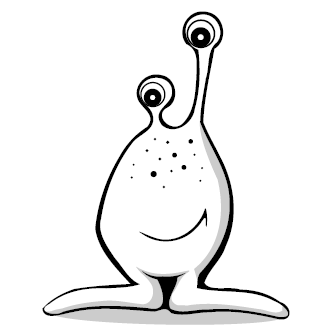
\includegraphics[width=\columnwidth]{opeolio.png}
\end{figure}
\subsection*{Hakeminen}
Aineenopettajan koulutukseen voi hakea
kolmella tavalla: hakeutumalla matematiikan, fysiikan
ja kemian opettajan kandi\-ohjelmaan päähaussa tai siirto\-haussa, tai täsmentämällä oman opinto-oikeutensa matematiikan, fysiikan ja kemian opettajan maisteri\-ohjelmaan heti kandi\-tutkinnon suorittamisen jälkeen (ns.\,maisterioptio). Matematiikan, fysiikan ja kemian opettajan kandiohjelmaan voidaan hyväksyä siirto\-haussa opiskelijaksi, jos hakija on suorittanut matematiikan, fysiikan tai kemian perusopinnot, ja jos hakija suorittaa hyväksytysti aineen\-opettajan valintakokeen. Jos sisäinen opettajuus herää vasta valmistumisen jälkeen, maisteri\-tutkinnon suorittanut voi hakea opinto-oikeutta erillisiin opettajan pedagogisiin opintoihin kerran vuodessa järjestettävässä haussa.

Aineenopettajan valintakoe on ryhmä- tai yksilö\-haastattelu. Haastattelun apuna saatetaan käyttää materiaalia, joka jaetaan haastattelun alussa. Haastattelun kesto on 20~minuuttia. Käytännössä hyväksyminen on lähes varmaa jos olet asiasta
kiinnostunut eikä sinulla ole rikos\-taustaa, joka tekisi sinusta soveltumattoman alalle -- onhan luonnon\-tieteiden
opettajista pulaa. Siirtohaku tapahtuu toukokuussa, ja ryhmä\-haastattelut pidetään kesäkuun alussa. Hakuohjeet löytyvät esimerkiksi Opinto\-polusta.

Kenties sinäkin
haluat tulevaisuudessa varmistaa työn
saannin? Parhaimmillaan opettajan opintojen
suorittaminen muiden maisterin\-opintojen
päälle vie vain yhden ylimääräisen vuoden
tai kaksi -- riippuen suunnitelmallisuudestasi. Opettajaksi kasvaminen vie kuitenkin aikaa, ja mitä aiemmin teet päätöksen ryhtyä opettajaksi, sitä parempi.
\subsection*{Opintojen rakenne}
Aineenopettajan opinnot koostuvat
periaatteessa kahdesta osasta: omassa koulutus\-ohjelmassa
tehtävästä opiskelusta ja pedagogisista
opinnoista, jotka sisältävät opetus\-harjoittelut. Näistä
ensimmäinen tarkoittaa siis omassa kandi- tai maisteri\-ohjelmassasi
tapahtuvaa opiskelua, joka sekin jakautuu
kahteen osaan. Ensimmäisenä opiskellaan
teoriaa, eli sitä samaa mitä kaikki
muutkin, vaikkapa fyysikolla mekaniikkaa,
aalto-oppia, termo\-fysiikkaa jne. Toinen
osuus taasen on lähinnä syventäviin opintoihin
kuuluvia kursseja, joissa opetetaan nimenomaan kyseisen aineen opettamista -- esimerkiksi käsitteen\-muodostusta sekä
kokeellisuutta. Pedagogiset opinnot ajoitetaan maisteri\-vaiheeseen, ja ne
suoritetaan Kasvatus\-tieteellisessä tiedekunnassa. Opetus\-harjoittelut tapahtuvat joko normaali\-kouluissa tai kenttä\-kouluissa.
\subsection*{Opiskelu}
Pedagogiset opinnot järjestää Kasvatus\-tieteellinen tiedekunta. Opinnot on järjestetty neljään eri periodiin yliopiston
periodien mukaisesti. Kukin periodi kannattaa
suorittaa yhden jakson aikana täysin;
seuraavan periodin kurssien osallistumis\-edellytyksenä
on pää\-sääntöisesti edellisen
periodin kurssien suorittaminen. Opinnot
on siis hyvä suorittaa numero\-järjestyksessä,
ensimmäisenä syys\-kuussa alkaa ensimäinen periodi. Periodien suorittamisen välillä on toki
mahdollista pitää taukoa, eikä kaikkia pedagogisia
opintoja ole välttämätöntä suorittaa
yhden vuoden aikana. Voi esimerkiksi suorittaa syksyn kaksi ensimmäistä periodia ensin ja vuoden päästä jatkaa kahden jälkimmäisen periodin kanssa.

Pedagogiset opinnot koostuvat aine\-didaktiikasta,
harjoittelusta ja muista opinnoista.
Opettajaopintojen suorittamisessa
kannattaa varautua koulumaisuuteen: miltei
kaikilla kursseilla on läsnä\-olo\-pakko, ja
opetus voi alkaa aamulla jo klo~8 ja kestää
lähes kellon ympäri. Kontakti\-opetuksen
lisäksi on tehtävä useita pieniä kirjallisia
töitä, kuten esseitä, sekä perehdyttävä oppi\-kirjoihin
ja muuhun materiaaliin. Lisäksi
ainakin aine\-didaktiikasta ja opetus\-harjoittelusta
tehdään port\-folio eli kansio, johon
kirjoitetaan itsearviointi sekä muuta pohdintaa
ja kerätään opintojen aikana tehtyjä
tehtäviä.
 
Opinnot voivat vaikuttaa raskailta,
mutta vastapainoksi opiskelijoiden yhteis\-henkeä
on pidetty hyvänä. Opintojen aikana
kannattaakin luoda suhteita kanssa\-opiskelijoihin,
sillä niistä lienee varmasti sekä
iloa että hyötyä tulevina opiskelu- ja työ\-vuosina.
Opettajan pedagogisten opintojen
käytännöistä ja kokemuksista opiskelijan
näkökulmasta kannattaakin myös kysellä
jo etukäteen vanhemmilta opiskelijoilta.
\subsection*{Aineenhallinnalliset opinnot}
Aineen\-hallinnalliset vaatimukset vaihtelevat
varsin laajasti riippuen ensimmäisestä
ja toisesta opetettavasta aineestasi. Esimerkiksi
fysiikassa ja kemiassa töihin kuuluu
opetus\-laboratorio\-töitä (kyllä -- kemian ja
fysiikan opettaja\-opiskelijat pääsevät suorittamaan
10~op ylimääräisiä laboratorioita!)
kun taasen matematiikassa opinnot ovat
hyvin pitkälti samaa kuin ei-opettaja\-opiskelijoillakin,
tosin erilaisella lähestymis\-tavalla.
Erilaisia aine\-vaatimuksia on yhtä
paljon kuin opetettavia aineitakin, joten
tarkempia tietoja varten käy kurkkaamassa
opetussuunnitelmaa hyvissä ajoin!

Tärkeintä on pitää huoli, että aineen\-hallinnallisia
kursseja on suoritettuna tarpeeksi
siirtyessä opetus\-harjoittelu\-vaiheeseen.
Yleisesti ottaen perus\-harjoittelu\-vaiheessa
ensimmäisestä opetettavasta aineesta tulee olla suoritettuna merkittävä
osa ja toisesta opetettavasta perusopinnot, ja syventävässä harjoittelussa
ensimmäisestä suoritettuna tulee olla jonkin
verran syventäviä opintoja ja/tai laboratoriotöitä, toisessa aineopintojen tulisi olla
paketissa.

\subsection*{Aineenopettajan koulutuspedagogiset opinnot (60~op)}
Suorittamalla kasvatustieteen perus- ja
aineopinnot eli opettajanpedagogiset
opinnot (60~op) saa aineenopettajan pätevyyden,
joka vaaditaan muun muassa perus\-opetuksen
ja lukion aineen\-opettajilta.
Opinnot suoritetaan maisterintutkinnon sivu\-tieteen\-alana. Käytännössä paino\-lasti jakautuu oikein ajoitettuna noin 50/50
keväälle ja syksylle.
\subsection*{Ainedidaktiikka}
Ainedidaktiikka on osana useissa pedagogisten opintojen kursseissa, joita ovat Opetuksen suunnittelu, toteutus ja arviointi, Opetus\-suunnitelma ja oppilaitoksen kehittäminen sekä Opettaja työnsä tutkijana. Aine\-didaktiikassa perehdytään omien
opettavien aineiden
opettamiseen luentojen ja pienryhmässä
tehtävien harjoitusten sekä keskustelujen
avulla. Käsittelyssä on muun muassa
opetus\-suunnitelma, oppitunnin pitäminen,
opetus\-materiaalit ja arviointi. Aine\-didaktiikkaan
kuuluu myös seminaarityön tekeminen kurssilla Opettaja työnsä tutkijana, eli
pienimuotoisen kasvatus\-tieteellisen tutkimuksen
tekeminen jostakin vapaasti valittavasta
aiheesta, joka liittyy opettavaan
aineeseen ja sen opettamiseen.
\subsection*{Opetusharjoittelu}
Opetus\-harjoitteluihin voi ilmoittautua
heti, kun aine\-opinto\-tasoisia kursseja on suoritettu riittävä
määrä. Harjoittelut tehdään pää\-sääntöisesti
Norsseissa, joissa jokainen harjoittelija saa kaksi
ohjaavaa opettajaa, yhden kummastakin
opetettavasta aineestaan. Perus\-harjoittelun
ohjaava opettaja on yleensä eri kuin
syventävän harjoittelun. Kullekin harjoitus\-tunnille
on tehtävä huolellinen tunti\-suunnitelma.
Käytännössä eri ohjaavien
opettajien vaatimat työmäärät vaihtelevat;
joku saattaa katsoa summittaisen tunti\-suunnitelman
tunnin aikana oppilaiden laskiessa,
kun taas toinen varaa keskusteluun
koko hyppy\-tuntinsa ja haluaa saada tarkan
suunnitelman. Muistathan varata riittävästi
aikaa tuntien suunnitteluun ja toteutukseen!

Varsinkin tieto\-tekniikan tunnit ovat yleensä
aiheista, joihin joutuu ensin itse tutustumaan,
jollei ole esimerkiksi Corel~Draw tai
Visual~Basic "-ekspertti. Ennen omia tunteja
kannattaa käydä seuraamassa opetus\-ryhmää
muiden aineiden tunneilla; näin oppii
tuntemaan luokan ja huomaamaan, minkälaisia
työtapoja siellä voi käyttää. Joissakin
luokissa saa helposti aikaan hyviä keskusteluja,
mutta toisissa kyselevää opetusta ei
kannata edes yrittää. Harjoitteluja pidetään
opettaja\-opintojen ehdottomasti antoisimpana
osana, josta kannattaa ottaa kaikki irti
-- toisin sanoen OPPIA!

\subsection*{Muut opinnot}
Muut opinnot pitävät sisällään neljä
kurssia yleisiä kasvatustieteen opintoja: Didaktiikka, Oppimisen psykologia, Kasvatuksen yhteis\-kunnalliset, kulttuuriset ja filosofiset perusteet sekä Oppimisen ja hyvin\-voinnin tuki. Kursseihin sisältyy pien\-ryhmä\-työskentelyä, jossa pyritään linkittämään kurssien sisältöä opettajan työhön.

Tentit pitävät sisällään esseiden kirjoittamista ja sähköisiä moni\-valintoja,
ja ne ovat suhteellisen helppoja.
Tentittävän materiaalin tarkka läpikäyminen
ei siis ole välttämätöntä. Maalais\-järjellä
ja omilla ajatuksilla pääsee pitkälle,
ja jos osaa laittaa jonkun kirjassa ja/tai luennolla
mainitun aiheeseen liittyvän teorian
ja kasvatus\-tieteilijän nimeen esseeseen,
pääsee huippu\-arvo\-sanoihin.

\subsection*{Opiskelupaikat}
Opetus järjestetään suurimmaksi osaksi
Kasvatus\-tieteellisen tiedekunnan tiloissa Silta\-vuoren\-penkereellä. Silta\-vuoren\-penkereeltä löytyy mm.\, Kasvatus\-tieteellisen
tiede\-kunnan kirjasto Minerva,
jossa on opiskelija\-tiloja, sekä Unicafe Olivia. Joitakin massaluentoja voi
olla keskusta\-kampuksellakin (Porthania, päärakennus).
Perus\-harjoittelu ja syventävä harjoittelu
suoritetaan pää\-sääntöisesti jommassa\-kummassa Helsingin yliopiston yliopiston
harjoittelu\-koulussa eli Norssissa.
Helsingin normaali\-lyseo sijaitsee Ratakadulla
ja Viikin norssi Viikissä. Yliopisto jakaa harjoittelu\-paikat.
\subsection*{Tiedotus}
Aineen\-opettajan pe\-da\-go\-gi\-si\-a opintoja
koskeva tiedotus (mm.\,ilmoit\-tautumiset,
tutkinto\-vaatimukset, opetus\-ajat ja -paikat,
tenttikirjat, muutokset sekä muu ajankohtainen
tiedotus) löytyvät WebOodista.

\vspace{0.5cm}\noindent
\textsc{HAO ry:n hallitus}\\
\textsc{Risto Karinkanta}\\
\textsc{Kaisa Väätäinen}

\twocolumn[\section{Aineenopettajan kursseja}]
\subsection*{Matematiikan opetuksen opinnot}
\subsubsection*{Perusopetuksen matematiikka (5~op)}
Perusopetuksen matematiikka "-kurssilla tutustutaan nimensä mukaisesti peruskoulun matematiikan opetuksen sisältöihin ja erilaisiin tapoihin oppia ja opettaa matematiikkaa. Sisältöihin perehdytään opetussuunnitelman perusteiden ja oppimateriaalien kautta. Kurssiin kuuluu lähiopetusta, ja lähiopetuskerroilla odotetaan aktiivista läsnäoloa. Työskentelytapoihin kuuluvat myös ryhmätyöt ja yhteinen keskustelu. 

Kurssin aikana aineenopettajaopiskelija muodostaa kuvaa itsestään opettajana ja vahvistaa käsitystään peruskoulussa opetettavista aiheista. Keskustelua rikastuttaa se, että kurssilla voi olla opiskelijoita hyvinkin erilaisista taustoista.
\subsubsection*{Matematiikkaa kaikkialla (5~op)}
Matematiikkaa kaikkialla "-kurssilla nähdään, miten matematiikka on osa meidän jokapäiväistä elämää ja käydään ryhmissä läpi monenlaisia matemaattisia ilmiöitä.	Kurssiin sisältyy luentoja, jotka ovat joka toinen viikko, netissä palautettavia monivalintatehtäviä, jotka ovat melko helppoja, sekä viikoittainen ``leikki''-ryhmä, jossa tarkastellaan matemaattisia luonnonilmiöitä. Kurssi kestää puoli vuotta mutta työmäärään nähden se ei ole yhtään hankala.
\subsubsection*{TVT matematiikan opetuksessa (5~op)}
Kurssi koostuu erilaisista matematiikan opetukseen liittyvistä osasuorituksista, joihin kuuluu esimerkiksi Geogebran käyttöä, symbolista laskentaa tietokoneohjelmistoilla tai ohjelmointia. Opiskelijana saat itse valita itseäsi kiinnostavia tai hyödyllisimmiksi kokemiasi aiheita. Osasuorituskursseilla opitaan paljon hyödyntämään esimerkiksi sähköisissä ylioppilaskirjoituksissa käytettäviä ohjelmistoja. 
\subsection*{Fysiikan opetuksen opinnot}
\subsubsection*{Didaktisen fysiikan kokeellisuus~I--II (5+5~op)}
Nämä kurssit painottavat kouluissa tehtäviä kokeellisia töitä ja niiden perustalle rakennettavaa opetusta. Kursseilla suunnitellaan ja toteutetaan sarja erilaisiin fysiikan aihealueisiin sopivia työsarjoja, joista kirjoitetaan työselostukset, jotka sisältävät graafisia esityksiä käsiterakenteista. Kursseihin kuuluu myös luennot, joilla esitellään kokeellisia töitä. 
\subsubsection*{Fysiikan käsitteenmuodostus~I: klassinen fysiikka (5~op)}
Käsitteenmuodostuksessa perehdytään fysiikan käsiterakenteisiin ja kehitetään kokonaisuuksien hallintaa fysiikan ilmiöistä. Kurssilla painotetaan sitä, miten käsiterakenteet ovat kehittyneet kokeellisilla töillä. Kurssin suorittamiseen kuuluu luento-osuus ja harjoitukset, joista osa tehdään verkko-opetuksena. Tehtäviin kuuluu keskusteluharjoituksia, joissa muun muassa reflektoidaan omaa oppimista ja kehitetään omaa osaamista harjoituksilla ja käsitekaavioilla.
\subsection*{Kemian opetuksen opinnot}
\subsubsection*{Kemia elinympäristössä (5~op)}
Kemia elinympäristössä (eli tuttavallisemmin KEY) "-kurssilla perehdytään siihen, millä keinoilla kemian opetuksesta saadaan mielenkiintoa herättävämpää esimerkiksi hyödyntämällä erilaisia oppimis\-ympäristöjä. Kurssilla tehdään vierailuja ja suurimpana työnä ryhmissä kehitetään oma kemiallinen koe peruskouluun tai lukioon sovellettavaksi. Koetta testataan ja kehitetään eteenpäin.
\subsubsection*{Kemian käsitteet ja ilmiöt opetuksessa (5~op)}
Kurssilla tutustutaan kemian perus\-opetuksen ja lukio-opetuksen opetussuunnitelmiin ja keskeisiin sisältöihin ja ilmiöihin ja suunnitellaan omia opetuskokonaisuuksia. Kuten muutkin kemian opetuksen kurssit, kurssi on hyvin opiskelijalähtöinen ja siellä pääsee paljon tekemään itse perinteisten luentojen lisäksi. Kurssilla tutustutaan myös opetuksessa käytettäviin TVT-sovelluksiin.
\subsubsection*{Tutkimuksellinen kemian opetus (5~op)}
Tutkimuksellinen kemian opetus- eli tuttavallisemmin Tutki-kurssilla harjoitellaan kokeellista ja tutkimuksellista työskentelyä opettajana työskentelyä varten. Kurssilla suunnitellaan kokeellisia töitä ja päästään myös toteuttamaan niitä käytännössä. Tämän lisäksi perehdytään myös kemikaalivaraston hoitamiseen, mikä useimmiten kuuluu kemian opettajan vastuualueisiin koulussa.
\end{document}